\documentclass[11pt]{article}
\usepackage[dvips]{graphics}
\usepackage{amssymb}
\usepackage{amsmath}
\usepackage{graphicx}
\usepackage{chicago}
\usepackage{rotating}
\usepackage{hyperref}
\usepackage{sectsty}

\addtolength{\topmargin}{-0.375in}
\addtolength{\oddsidemargin}{-0.35in}
\addtolength{\evensidemargin}{-0.35in}
\addtolength{\textheight}{0.5in}
\addtolength{\textwidth}{0.5in}
\addtolength{\parskip}{0.05in}
\renewcommand{\baselinestretch}{1.5}
\newcommand{\vsp}{\vspace{\baselineskip}}
\newcommand{\be}{\begin{equation}}
\newcommand{\ee}{\end{equation}}
\newcommand{\gr}[1]{\ensuremath  {\frac{\dot {#1}}{#1}}}

\begin{document}
\renewcommand{\baselinestretch}{1}
\author{{\Large Valentin Bolotnyy} \\
Federal Reserve Board\thanks{E-mail: valentin.bolotnyy@frb.gov.\vspace{0.05in}} \and
{\Large Rochelle M. Edge} \\
Federal Reserve Board\thanks{E-mail: rochelle.m.edge@frb.gov.\vspace{0.05in}}\and
{\Large Luca Guerrieri} \\
\addtocounter{footnote}{5} Federal Reserve Board\thanks{%
E-mail: luca.guerrieri@frb.gov.}}
\title{\textbf{Stressing Bank Profitability for Interest Rate Risk}}
\date{\today}
\maketitle


\begin{abstract}
\vspace{-0.06in} \noindent  Regular bank stress testing (and the capital planning that it implies) is one of the three complementary reforms that has been made to U.S. capital regulation in response to the shortcomings of the pre-crisis regime.
 The form of stress testing mandated under the Dodd-Frank Act for the Federal Reserve to undertake and the form being used by the Federal Reserve for its annual Comprehensive Capital Analysis and Review (CCAR) is one based around a small number of scenarios.  This approach involves specifying macroeconomic and financial scenarios that represents stressful conditions over the time horizon of the stress test and then projecting, for each BHC in the stress test, its losses, income, and path of capital \textit{given that scenario}. In this paper, we focus on the revenue generate aspect of banks and consider the ability of empirical models to translate developments in interest rates into bank net interest margins (NIMs). We consider an extensive number of time-series models. While our best-performing models beat a no-change forecast, the confidence bands are so large that baseline and stress scenarios taken from CCAR appear indistinguishable.


\vspace{.125in}

\noindent Key Words:

\vspace{.125in}

\noindent JEL Classification: To be completed.


\end{abstract}
\renewcommand{\baselinestretch}{1.5}
\thispagestyle{empty}

\newpage
\setcounter{page}{1}

\section{Introduction}

\vspace{-0.1in}
Regular bank stress testing (and the capital planning that it implies) is one of the three complementary reforms that has been made to U.S. capital regulation in response to the shortcomings of the pre-crisis regime.\renewcommand{\baselinestretch}{1}\footnote{See Governor Tarullo’s November 2011 speech ``The Evolution of Capital Regulation'' for this characterization of stress testing. The two other reforms that he mentions are improvements to the traditional, individual firm approach to capital regulation and the introduction of a macroprudential component to capital regulation.\vspace{0.05in}}\renewcommand{\baselinestretch}{1.5} While stress testing can take many forms---for example, being based on a small number of scenarios, being based on a large number of scenarios, or even being undertaken in reverse form to achieve a certain adverse outcome---the form of the stress tests mandated under the Dodd-Frank Act for the Federal Reserve to undertake and the form being used by the Federal Reserve for its annual Comprehensive Capital Analysis and Review (CCAR) is one based around a small number of scenarios.  This approach involves specifying a small number of macroeconomic and financial scenarios that represents stressful conditions over the time horizon of the stress test and then projecting, for each BHC in the stress test, its losses, income, and path of capital \textit{given that scenario}. Clearly, there are at least two important parts to conducting bank stress tests (i)~formulating macroeconomic and financial scenarios that should be stressful to banks and (ii)~developing econometric models that are able to translate such stressful conditions into losses, income, and capital.
%This paper considers the latter of these two issues; that is, translating
%stressful economic conditions into bank income.

In developing econometric models to translate stressful economic conditions into key bank financial-statement variables it is important to consider what types of developments are likely to be stressful to banks and what particular economic variables are likely to capture these stresses. It is then critical that the models being used for stress testing are able to translate developments in these economic variables into the key bank financial-statement variables that the model is designed to project.  In this paper, we examine this property for models of bank net interest margins (NIMs), defined as the ratio of net interest income (NII) to interest earning assets, where NII is the difference between a bank's interest income and interest expenses.

Our motivation for focusing on models of NIMs is based on a number of considerations. First, bank losses that arise from banks' having to pay out more in interest on their liabilities than they are earning from their assets should not be overlooked as an important source of risk to the banking and broader financial sector.  To be sure, losses that arise from this source of risk---called, interest rate risk---were much less prominent in the most recent crisis relative to bank losses that stem from loan defaults---that is, credit risk---but there are ample examples of other earlier banking crises in which adverse developments in NIMs have played a significant role.  The most familiar of these from the U.S. perspective is the Savings and Loans (S\&L) crisis that started in the early 1980s with short-term interest rates rising above long-term interest rates---in part, as a result of the Volcker disinflation.  This resulted in interest expenses rising above interest income, NII and NIMs turning negative (in the thrift sector), and sizable losses and ultimately a substantial number of bank failures.  Likewise, the Nordic banking crises of the late 1980s and early 1990s (for Finland, Sweden, and Norway)---which represent three of Reinhart's and Rogoff's~(2009) ``big five'' banking crises---were associated with elevated short-term interest rates that depressed NII and NIMs and lead to sizable bank losses and failures. In the Nordic crises, high short-term interest rates resulted from these countries attempting to maintain currency pegs with the Deutschemark in the face of the tight German monetary policy that accompanied its loose fiscal policy associated with re-unification spending. Finally, there is also the U.K.'s secondary banking crisis of the early 1970s, which was associated with a sudden increase in short-term interest rates that abruptly drove up banks' costs of funds so too leading to bank losses and failures.  To be sure, large increases in short-term rates and declines in net interest income were not the \textit{only} reason for any of these crises---indeed, there was at least one major class of asset prices that collapsed in each of these crises---but short-term interest rates---and, in particular, their elevated levels relative to long-term interest rates---were significant and in most cases equivalent in importance to the other causes of the crisis.

Another motivation for our focus on models of NIM stems from the recent lackluster pace of bank profit growth, which is becoming an increasing source of concern to market commentators and regulators alike. Bank net income growth in recent years has been largely supported by unsustainable cost cutting and reductions in provisioning, rather than from sources like NII.  NII growth, for example, (in both nominal and real terms) has been well below average in recent years while NIMs (NII relative to interest earning assets) have also been depressed.%\renewcommand{\baselinestretch}{1}\footnote{We should probably show both these  charts with adjustments for FAS 167.\vspace{0.05in}}\renewcommand{\baselinestretch}{1.5}  
Given their already low level, any adverse development that puts further downward pressure on NIMs could be very stressful for banks and, as such, it is important that the economic developments (likely involving interest rates) that would drive these outcomes are well-modeled.

Our final motivation for examining NIMs is that despite the importance of NIMs for the financial condition of banks \textbf{[and the attention that it receives from bank equity analysts]}, the modeling of NIMs has received much less attention in the risk-modeling literature relative to the modeling of bank variables related to credit risk.  To be sure, the recent increase in the importance of stress testing has led to the development of a number of models that link NIMs to macroeconomic variables---such as, short-term Treasury rates and the slope of the Treasury yield curve---with Kovner \textit{et al}.~(2011) and Covas \textit{et al}.~(2012) being two notable examples for the U.S.  However, this research places relatively less emphasis on the conditional forecasting properties of these models, which is important given that these models are ultimately to be used to project bank losses, income, and capital given macroeconomic scenarios.\renewcommand{\baselinestretch}{1}\footnote{Covas \textit{et al}. do present some forecast evaluation results in order to demonstrate the benefits of focusing on quantile projections. However, they only report results for net chargeoffs and pre-provisioning net revenue and their focus is on density forecast evaluation.\vspace{0.05in}}\renewcommand{\baselinestretch}{1.5}

In summing up our motivation on the importance of modeling NIMs and studying interest rate risk, we would also note that the Federal Reserve chose to feature interest rate risk in one of the scenarios specified for the 2013 Dodd-Frank Act (DFA) stress tests.  In particular, for the 2013 DFA stress tests, the Federal Reserve specified the adverse scenario as one in which the Treasury yield curve shifted up and flattened.  As noted by the Federal Reserve in its (proposed) Policy Statement on scenario design, the Board varies ``the approach it uses for the adverse scenario each year so that the results of the scenario provide the most value to supervisors, in light of current condition of the economy and the financial services industry.''

In this paper we examine how well a range of time-series models can explain NIMs. We emphasize the models' pseudo-out-of-sample \textit{conditional} forecast performance. We adopt this pseudo-out-of-sample approach for the simple reason that the evaluation of models based on their in-sample forecast performance, frequently leads to the econometrician over-fitting the model within the sample so as to maximize in-sample forecast performance. We focus on conditional forecasts for the reason that scenario-based stress testing of the banking system is the underlying motivation for our analysis and it is along the dimensions of \textit{conditional} forecasts that model forecast performance is important.  Focusing on conditional forecast performance also means that we can separate the task of modeling and forecasting NIMs from that of forecasting interest rates, which is itself a sizable topic (see Duffee, 2012).

In determining which variables to include in our model of NIMs we look to the variables that have been emphasized by two existing literatures on NIMs.  The first literature emphasizes the link between interest rates of different maturities and NIMs and is more in the macro-banking tradition. The second literature focuses on the optimal margin set by banks based on considerations like the competitive structure of the lending and deposit markets in which the bank participates, the degree of managerial risk aversion, and the degree of uncertainty associated with the future path of interest rates and is much more in the micro-banking tradition.  

We proceed as follows. Section~two provides a review of the literature on NIMs with an eye to cataloguing variables that have been found useful to explain the evolution of NIMs. Section~three turns to the models that we develop to forecast NIMS. Section 4 concludes.

\section{Related literature}

\vspace{-0.1in}
There are primarily two empirical literatures on modeling NIMs.  The first literature emphasizes the link between interest rates of different maturities and NIMs and lies more in the macro-banking tradition.  The second literature focuses on the optimal margin set by banks and lies more in the micro-banking tradition.

The papers for the U.S. by Kovner \textit{et al}. and Covas \textit{et al}. noted earlier fall into the category of papers in the macro-banking tradition, where in both cases these models link NIMs to  a measure of the slope of the yield curve and a measure of short-term market rate.  Banks' earnings from interest income reflect two key services that banks supply---maturity transformation services (that is, borrowing short and lending long) and deposit transactions services---and the returns to these services are reflected by these two interest rate variables.  The slope of the yield curve reflects the return to banks from maturity transformation and thus is expected to enter NIM models with a positive sign. The short-term market rates in NIM models reflect the fact that bank deposit rates, while typically lower (since they provide transactions services), are constrained by the zero lower bound.  As such, the short rate places an upper limit on what banks can earn from the provision of their transactions services. As a result, the short rate is expected to enter the model, also, with a positive sign.

Both Kovner \textit{et al}. and Covas \textit{et al}. measure the slope of the yield curve in their respective NIM models with the 10-year to 3-month Treasury term spread and short-term market rates with the 3-month Treasury bill rate, as do English~(2002) and English \textit{et al}.~(2012)---two other papers in this tradition.  All of these papers estimate NIM models with slightly different purposes in mind.  The NIM models estimated by Kovner \textit{et al}. and Covas \textit{et al}. are developed for stress testing and are part of much larger aggregative models of a number of components of banks' financial statements. These models are both estimated on panel data with the most notable difference between these models being the estimation techniques they employ: Least squares regression in the case of Kovner \textit{et al}. and quantile regression in the case of Covas \textit{et al}.

Like our paper, English also only studies NIMs, although he does so for a number of countries (that is, all G-7 countries except for France, and for Australia, Norway, Sweden, and Switzerland).  Addditionally, (and as we also do later), he considers asset yields and liability yields separately---the two measures that when differenced imply NIMs.  English's main focus is understanding how well the aggregate banking sectors in the countries he studies appear to have managed the interest rate risk that they face on their earnings, as such he uses aggregate data (rather than firm-level data) and does not focus on the conditional forecasting performance of his model.

Finally, English \textit{et al} consider the relationship between NIMs and the slope of the yield curve and short-term rates for a panel of banks, however, in contrast to the other studies they allow for the specific coefficients estimated for each bank to vary as linear functions of bank balance sheet ratios that one \textit{a priori} might think would be relevant to net interest income.  In particular, these ratios include the maturity gap between bank assets and liabilities, the deposit share of liabilities, and the loan share of assets. Again, since English \textit{et al} are focussed on understanding the determinants of NIMs they do not consider conditional forecast performance.

  A separate strand of the NIM modeling literature comes from the micro-banking tradition, which focuses on the determinants of the loan rates and deposit rates that banks set as implied by the maximization of their profits. Papers in this tradition---such as, Ho and Saunders~(1981), Angbazo~(1997), and Saunders and Schumacher~(2000)---are based around what is known as the ``dealership'' model of banks; that is, banks in these models are viewed as dealers in the credit market, acting as an intermediary between demanders and suppliers of funds.  Banks are modeled as being able to raise funds from and lend funds to short-term money markets as well as being able to raise deposits from and make loans to nonfinancial agents.

In borrowing or lending in money markets banks face a market rate, which can vary over time, while in raising deposits from or extending loans to nonfinancial agents banks have the ability to set rates.  In raising deposits, banks can pay a below market rate that is fixed for the full life of the deposit and in extending loans they can earn an above market rate that is also fixed for the full maturity of the loan.  Importantly, the life of the deposit is the same as that of the loan, reflecting the fact that while core deposits can, in principal, be withdrawn on demand from a bank they are in practice extremely sticky.  Interest rate risk arises in this model from the fact that deposit-taking and lending opportunities do not arrive at the bank at precisely the same time but rather arrive at any time with some probability, where these probabilities---which are different for deposits and lending opportunities---depend on the interest rates set by the bank on deposits and loans.  Consequently, banks can find themselves holding deposits without loans, that they must then invest at variable market rates (and that could adversely fall below the deposit rate), or loans without deposits, that they must then fund at variable market rates (that could adverse rise above the lending rate).

The solution to the bank's profit-maximization problem is the spread between the loan rate and the deposit rate and this has two parts. The first part is the spread that a bank would set if it were completely risk neutral. This depends only on the degree of competition faced by the bank in the loan markets and the deposit markets in which it operates, where, in the model, this is captured by the slope of the loan demand schedule and slope of the deposit supply schedule facing the bank. The second part of the spread reflects banks' risk aversion to the situation of either having deposit supply without corresponding loan demand or having loan demand without the corresponding deposit supply. Consequently, the second part of the spread is the compensation for this risk that banks require in order for them to be willing to take deposits and lend. This depends positively on the banks' degree of risk aversion as well as the volatility of interest rates.

In Ho and Saunders the degree of competition faced by the bank in loan and deposit markets does not enter their estimated model, since they argue that this variable is quite slow moving and their analysis is undertaken only over a period of three years.  Saunders and Schumacher do consider the degree of competition in their analysis--which is cross-country in nature---although this takes the form of a country dummy variable in the regressions. In all cases the banks' degree of risk aversion does not enter the specification for estimated models of NIMs since this is difficult to measure, although the volatility of interest rates does and this is measured by the annual or quarterly standard deviation of weekly Treasury rates of different maturities (\textit{e.g.}, 3-month, 1-year, 2-year, 3-year, and 5-year rates).

Most papers in this literature also add a few more controls to the model before estimation, although in all cases this is done in a fairly \textit{ad hoc} way.  These variables include banks' payments of implicit (instead of, explicit) interest on deposits;\renewcommand{\baselinestretch}{1}\footnote{This takes place through service charge remissions and other types of depositor subsidies due to regulatory restrictions of explicit interest payments and is measured by the difference between noninterest expenses and noninterest revenue, all divided by interest earning assets.\vspace{0.05in}}\renewcommand{\baselinestretch}{1.5} banks' non-interest-bearing reserve requirements;\renewcommand{\baselinestretch}{1}\footnote{This captures the influence of the economic cost of funds over and above the published interest expense and is measured by non-interest bearing reserves divided by total assets.\vspace{0.05in}}\renewcommand{\baselinestretch}{1.5} banks' default risk, since this should imply an additional premium charged on the rate of the banks loans given the potential loss in bank capital;\renewcommand{\baselinestretch}{1}\footnote{This is measured by net chargeoffs divided by total loans.\vspace{0.05in}}\renewcommand{\baselinestretch}{1.5} and, bank capital, since capital is costly and banks with higher capital may seek to cover this with higher lending rates.  Note that all of the empirical analysis in the ``dealership'' model literature for studying NIMs is undertaken at the firm-level and as such many of the \textit{ad hoc} controls that are added to the model are included so as to address cross-firm differences.

We would note that Angbazo does add default risk to the bank's profit-maximization problem and, as such, default risk does enter his model of NIMs in a more rigorous way.  Here he finds that for money center banks net interest margins are more sensitive to default risk than they are to interest-rate risk, while super-regional and regional banks are sensistive to interest-rate risk but less so to default risk. These findings he notes are consistent with these money center banks' greater concentration of short-term assets and greater use of off-balance sheet (OBS) hedging instruments.

There is a further strand of the micro-banking literature looking at determinants of banks' NIMs---which includes papers by Zarruk~(1989) and Wong~(1997)---that we mention but do not discuss at length.  In these models deposits and lending opportunities arrive at the same time and depend on the deposit and loan rates being set by banks but there is some stochastic element to the volume of deposits that banks will raise given the interest rate they set, thus requiring the banks in the model, who are risk average, to borrow or lend in the federal funds market.  These models also include features like administrative costs on deposits and loans as well as costs associated with deposit insurance premia and the primary use of these models is for comparative static exercises that examine how changes in these parameters---as well as considerations like uncertainty---will affect bank spreads.  Utlimately, however, these papers are not empirical and since the majority of their theoretical findings confirm those of those of papers like Ho and Saunders, Angbazo, and Saunders and Schumacher, we do not delve too deeply into them here.

In summing up our review of other empirical analyses of NIMs a few variables stand out---in addition, to short- and long-term interest rates---as relevant for our analysis.  The degree of competition faced by the bank in the loan markets and the deposit markets in which it operates stands out as an important consideration, especially given that the sample we use in our analysis is much longer than the samples considered by Ho and Saunders, Angbazo, and Saunders and Schumacher.  Interest rate volatility, also appears important, since this has likely also changed over our sample.  The other variables that previous authors in the micro-banking tradition have added to their models in an \textit{ad hoc} way we hold-off for the time being from adding to our analysis.  This is largely because our analysis at this stage is at the aggregate level and these additional variables appear to have been added to explain variations in NIMs across firms.

\section{Models for forecasting NIMs}

\vspace{-0.1in}
\noindent \textbf{1. Simple forecast combination.} We regress NIMs on each yield $r(\tau )_{t-1}$ separately: \
\[
NIM_{t}=c_{\tau }+\rho _{\tau }NIM_{t-1}+\gamma _{\tau }r(\tau )_{t-1}+{\eta
_{\tau ,t}}
\]

Each regression is use to produce an $s$ step-ahead forecast of NIMs conditional on yields on treasuries with maturity $\tau $ observed through period $t+s-1.$ This conditional forecast is denoted by $NIM_{\tau ,t+s/t}.$ The simple forecast comnination is then given by:
\[
NIM_{t+s/t}=\sum_{\tau }\frac{NIM_{\tau ,t+s/t}}{N},
\]
where $N$ is the number of maturities considered.

\noindent \textbf{2. A dynamic factor model for NIMs.} Using the state space representation, the state equations of our restricted dynamic factor model is given by
\[
\left(
\begin{array}{c}
{L_{t+1}-\mu _{L}} \\
{S_{t+1}-\mu _{S}} \\
{C_{t+1}-\mu _{C}} \\
\widehat{NIM}_{t+1}-\mu _{\widehat{NIM}}%
\end{array}%
\right) {\normalsize \ =\ }\left(
\begin{array}{cccc}
a_{11} & a_{12} & a_{13} & 0 \\
a_{21} & a_{22} & a_{23} & 0 \\
a_{31} & a_{32} & a_{33} & 0 \\
a_{41} & a_{42} & a_{43} & a_{44}%
\end{array}%
\right) {\normalsize \ }\left(
\begin{array}{c}
{L_{t}-\mu _{L}} \\
{S_{t}-\mu _{S}} \\
{C_{t}-\mu _{C}} \\
\widehat{NIM}_{t}-\mu _{\widehat{NIM}}%
\end{array}%
\right) {\normalsize +}\left(
\begin{array}{c}
{\eta _{Lt}} \\
{\eta _{St}} \\
{\eta _{Ct}} \\
{\eta _{NIMt}}%
\end{array}%
{\normalsize \ }\right) ,
\]
where $L_{t},S_{t},$ and $C_{t}$ are level slope and curvature factors for the yield curve, respectively, and $\widehat{NIM}_{t}$ represent a measure of NIMs cleaned of observation error. The term $\mu _{x}$ denotes the mean of $x$. The terms ${\eta _{Lt}}$, ${\eta _{St}}$, ${\eta _{Ct}}$, ${\eta_{NIMt}}$ denote independently distributed innovations with joint covariance matrix $\Omega $.

The observation equations, which relate a set of $N$ yields (in our case, 12) and observed NIMs can be split into two groups. In the first group, equations for yields on treasuries of maturity $\tau $ take the form:
\[
r(\tau )=\left(
\begin{array}{cccc}
1 & \frac{1-e^{-\lambda \tau }}{\lambda \tau } & \frac{1-e^{-\lambda \tau }}{%
\lambda \tau }-e^{-\lambda \tau } & 0%
\end{array}%
\right) \left(
\begin{array}{c}
{L_{t}-\mu _{L}} \\
{S_{t}-\mu _{S}} \\
{C_{t}-\mu _{C}} \\
\widehat{NIM}_{t}-\mu _{\widehat{NIM}}%
\end{array}%
\right) +e(\tau )_{t},
\]%
where $e(\tau )_{t}$ is i.i.d. measurement error assumed to be uncorrelated
across observations. \bigskip In the second group, the equation for observed
NIMs takes the form%
\[
NIM_{t}=\left(
\begin{array}{cccc}
0 & 0 & 0 & 1%
\end{array}%
\right) \left(
\begin{array}{c}
{L_{t}-\mu _{L}} \\
{S_{t}-\mu _{S}} \\
{C_{t}-\mu _{C}} \\
\widehat{NIM}_{t}-\mu _{\widehat{NIM}}%
\end{array}%
\right) +e(NIM)_{t},
\]
where $e(NIM)_{t}$ is i.i.d. measurement error assumed to be uncorrelated across observations.

Out-of-sample conditional forecasts for NIMs from this model, are obtained using the Kalman filter.

\noindent \textbf{3. Dynamic factor model with second-step regression for NIMs.} The dynamic factor model we consider takes the form
\[
\left(
\begin{array}{c}
{L_{t+1}-\mu _{L}} \\
{S_{t+1}-\mu _{S}} \\
{C_{t+1}-\mu _{C}}%
\end{array}%
\right) {\normalsize \ =\ }\left(
\begin{array}{ccc}
a_{11} & a_{12} & a_{13} \\
a_{21} & a_{22} & a_{23} \\
a_{31} & a_{32} & a_{33}%
\end{array}%
\right) {\normalsize \ }\left(
\begin{array}{c}
{L_{t}-\mu _{L}} \\
{S_{t}-\mu _{S}} \\
{C_{t}-\mu _{C}}%
\end{array}%
\right) {\normalsize +}\left(
\begin{array}{c}
{\eta _{Lt}} \\
{\eta _{St}} \\
{\eta _{Ct}}%
\end{array}%
\right)
\]

\[
r(\tau )=\left(
\begin{array}{ccc}
1 & \frac{1-e^{-\lambda \tau }}{\lambda \tau } & \frac{1-e^{-\lambda \tau }}{%
\lambda \tau }-e^{-\lambda \tau }%
\end{array}%
\right) \left(
\begin{array}{c}
{L_{t}-\mu _{L}} \\
{S_{t}-\mu _{S}} \\
{C_{t}-\mu _{C}} \\
\widehat{NIM}_{t}-\mu _{\widehat{NIM}}%
\end{array}%
\right) +e(\tau )_{t},
\]

We obtain smoothed estimates of the factors $L_{t},S_{t},$ and $C_{t}$ conditional on information up until period $T.$ We estimate two alternative second-step forecasting equations:

\noindent \textbf{Alternative a. Multivariate} (all yield curve factors included in one NIM equation)
\[
NIM_{t}=c+\rho NIM_{t-1}+\gamma _{L}L_{t-1}+\gamma _{S}S_{t-1}+\gamma
_{C}C_{t-1}
\]

\noindent \textbf{Alternative b. Forecast combination} (each factor included in a separate equation and forecasts from each equation combined)
\[
NIM_{t}=c_{i}+\rho _{i}NIM_{t-1}+\gamma _{i}F_{i,t-1}+{\eta _{i,t},}
\]%
where $F_{i}\in \left\{ L,S,C\right\} .$ Forecasts $NIM_{i,t+s/t}$ from each separate regression are then aggregated as:

\[
NIM_{t+s/t}=\sum_{i}\frac{NIM_{i,t+s/t}}{3},
\]

\noindent \textbf{4. Forecast combination with observed factors.} Define $\left\{L,S,C \right\} ,$ the observed factors as in subsection 3.1 above.
\[
NIM_{t}=c_{i}+\rho _{i}NIM_{t-1}+\gamma _{i}O_{i,t-1}+{\eta _{i,t},}
\]%
where $O_{i}\in \left\{ L,S,C\right\} .$ Forecasts  from each separate regression, $NIM_{i,t+s/t},$are then aggregated as:

\noindent \textbf{5. VAR with observed factors.} Define level factor to coincide with the 10-year yield; define the slope factor as the difference between the 10-year and the 3-month yields; define the curvatures factor to be 2 times the 2-year yield minus the the sum of the 3-month and 10-year yields. The VAR of order four includes the three observed factors defined as above and NIMs. Forecasts conditional on the factors are obtained using the Kalman filter.
\[
NIM_{t+s/t}=\sum_{i}\frac{NIM_{i,t+s/t}}{3},
\]

\noindent \textbf{6. No-change forecast.} According to this model $NIM_{t+s/t}=NIM_{t}${\normalsize . }


%\renewcommand{\baselinestretch}{1}\footnote{...\vspace{0.05in}}\renewcommand{\baselinestretch}{1.5}

\section{Data}

\vspace{-0.1in}

\subsection{Net interest margins}

\vspace{-0.1in} The data on bank net interest margins (NIMs) that we use is from the quarterly Consolidated Reports of Condition and Income (Call Report) that every national, state member, and insured nonmember bank is required to file on the last day of each quarter by the Federal Financial Institutions Examination Council (FFIEC). The Federal Deposit Insurance Corporation is tasked as the overseer, collecting and reviewing all submissions. Call Report data used in this analysis are cleaned and adjusted for bank mergers and acquisitions, using structure data from the National Information Clearinghouse (NIC) on mergers and acquisitions. Foreign entities are excluded and domestic subsidiaries are aggregated up to the parent, bank-holding-company (BHC), level.\renewcommand{\baselinestretch}{1}\footnote{NIM data are adjusted for mergers between commercial banks by comparing balance sheet values of interest income, interest expenses, and interest-earning assets at the end of the quarter with those at the beginning of the quarter, accounting for amounts acquired or lost during the period because of mergers. For information on the merger-adjustment procedure for income, see the appendix in English and Nelson (1998).\vspace{0.05in}}\renewcommand{\baselinestretch}{1.5}

NIMs in our models are expressed as the annualized percentage of net interest income over interest-earning assets. To get an aggregate banking sector measure of NIMs, we aggregate NIMs for the top 25 BHCs, as ranked by total assets, which is assessed quarterly.

\subsection{Treasury yields}

The yields data are derived using a smoothing technique from Gurkaynak, et al. (2007), based on Nelson and Siegel (1987) and Svensson (1994), which allows for daily measures of an off-the-run Treasury yield curve. We use yields for twelve maturities in our models: 3 month, 6 month, 9 month, 1 year, 2 year, 3 year, 5 year, 7 year, 10 year, 15 year, 20 year, and 30 year.\renewcommand{\baselinestretch}{1}\footnote{Daily yields are published with a two-day lag under the base mnemonic SVENY at  www.federalreserve.gov/econresdata/researchdata/feds200628\_1.html.\vspace{0.05in}}\renewcommand{\baselinestretch}{1.5} The yields included are quarterly averages of daily yields.  The data on NIMs and yields start in 1985Q4 and end in 2008Q2, a period that stops short of the interest rate regime shift to the zero lower bound.

\subsection{Micro-banking variables}

\vspace{-0.1in} The main variable that we use to capture the degree of competition that banks face is the size of the traditional
banking industry (as measured by the assets in that industry) relative to the size of the total banking industry, that is, both
traditional and shadow banking (as measured by the combined assets of these these two industries). We use this measure for the
reason that competition from the shadow banking sector is the most relevant form of increased competition faced by the
traditional banking sector.  Importantly, competition from the shadow banking sector affects both sides of traditional banks'
balance sheets. For example, it puts upward pressure on the deposit rate that traditional banks must pay to attract deposits---since the shadow banking sector offers alternatives to deposits like money market mutual funds---and it puts downward pressure on the lending rate that traditional banks can earn---since the shadow banking sector offers alternatives to bank loans like loans from finance companies. This measure can be easily calculated from the U.S. Financial Accounts (previously known as the Flow of Funds Accounts), where the traditional banking sector consists of commercial banks, savings institutions, and credit unions and the shadow banking sector consists of broker-dealers, ABS issuers, finance companies, mortgage pools, and funding corporations.

In papers that have modeled NIMs as a function of more microeconomic variables interest rate volatility has been measured by
the quarterly variance of weekly Treasury interest rate series. (See, for example, Ho and Saunders, 1981, and Saunders
and Schumacher, 2000.)  Typically, also, it is the quarterly variance of several Treasury interest rate series that are
considered---such as, the 3-month rate, 1-year rate, 2-year rate, 3-year rate, and 5-year rate---with the best fitting series then
included in the regression.  We also consider the Merrill Lynch MOVE index, which is the bond market equivalent to the VIX.

% Suggestion to look at the MOVE index.  It looks like it goes back to at least April 1988 (http://www.businessinsider.com/the-move-index-bonds-2010-3) This (http://business.financialpost.com/2012/11/01/investors-seeking-yield-should-use-move-and-vix/) also says it was created in 1988.


\newpage
\begin{thebibliography}{99}
\vspace{-0.1in}
\bibitem{abel82} Abel, A.B. (1982).  ``Dynamic Effects of Permanent and Temporary Tax Policies in
a $q$ Model of Investment.''  \textit{Journal of Monetary Economics}, 9, 353-373.

\bibitem{auerb1} Auerbach, A.J. (1979). ``Wealth Maximization and the Cost of Capital.''
\textit{Quarterly Journal of Economics}, 93, 433-446.

\bibitem{auerb2} Auerbach, A.J. (1989). ``Tax Reform and Adjustment Costs:  The Impact on
Investment and Market Value.''  \textit{International Economic Review}, 30, 939-962.

\bibitem{auerb3} Auerbach, A.J., and L.H. Summers (1979). ``The Investment Tax Credit: An Evaluation.''
NBER Working Paper No.~404.

\end{thebibliography}


\newpage
{\normalsize \clearpage
\begin{sidewaystable}
\center
\caption{RMSE for shortened sample: 1989Q2-2008Q2}
\begin{tabular}{|l|c|c|c|c|c|c|c|c|c|c|}
\hline
&Step 1 &Step 2 &Step 3 &Step 4 &Step 5 &Step 6 &Step 7 &Step 8 &Step 9 &Step 10\\
\hline
1. Simple Forecast Combination             &0.107&0.133&0.148&0.168&0.187&0.202&0.213&0.209&0.216&0.223\\
2. DFM                                     &0.122&0.148&0.169&0.212&0.247&0.278&0.316&0.340&0.373&0.404\\
3a. DFM with 2nd Step Regression           &0.118&0.167&0.209&0.260&0.308&0.356&0.398&0.433&0.474&0.511\\
3b. DFM with Forecast Combination          &0.112&0.159&0.199&0.247&0.300&0.351&0.399&0.438&0.489&0.535\\
4. Forecast Combination of Observed Factors&0.118&0.169&0.216&0.273&0.336&0.399&0.456&0.509&0.567&0.622\\
5. VAR on Observed Factors                 &0.166&0.209&0.263&0.302&0.342&0.375&0.380&0.430&0.451&0.499\\
6. No-Change Forecast                      &0.107&0.138&0.154&0.181&0.206&0.228&0.244&0.248&0.271&0.293\\
\hline
\end{tabular}
\end{sidewaystable}
}

\newpage
{\normalsize \clearpage
\begin{sidewaystable}
\caption{RMSEs over full sample: 1985Q4-2008Q2}
\center
\begin{tabular}{|l|c|c|c|c|c|c|c|c|c|c|}
\hline
&Step 1 &Step 2 &Step 3 &Step 4 &Step 5 &Step 6 &Step 7 &Step 8 &Step 9 &Step 10\\
\hline
1. Simple Forecast Combination             &0.105&0.140&0.164&0.191&0.218&0.244&0.265&0.281&0.305&0.327\\
3a. DFM with 2nd Step Regression           &0.128&0.190&0.244&0.299&0.350&0.397&0.438&0.475&0.514&0.549\\
3b. DFM with Forecast Combination          &0.112&0.158&0.197&0.240&0.290&0.337&0.373&0.407&0.446&0.480\\
4. Forecast Combination of Observed Factors&0.116&0.174&0.227&0.284&0.347&0.409&0.459&0.508&0.554&0.595\\
5. VAR on Observed Factors                 &0.148&0.196&0.243&0.275&0.283&0.296&0.319&0.377&0.456&0.530\\
6. No-Change Forecast                      &0.107&0.138&0.154&0.181&0.206&0.228&0.244&0.248&0.271&0.293\\
\hline
\end{tabular}
\end{sidewaystable}
}

\newpage
{\normalsize \clearpage
\begin{sidewaystable}
\caption{RMSEs for models that include the share of asset of the shadow banking sector. Estimation sample: 1989Q2-2008Q2}
\center
\begin{tabular}{|l|c|c|c|c|c|c|c|c|c|c|}
\hline
&Step 1 &Step 2 &Step 3 &Step 4 &Step 5 &Step 6 &Step 7 &Step 8 &Step 9 &Step 10\\
\hline
1. Simple Forecast Combination             &0.110&0.143&0.165&0.192&0.222&0.248&0.267&0.274&0.287&0.300\\
3a. DFM with 2nd Step Regression           &0.121&0.170&0.212&0.262&0.312&0.360&0.403&0.436&0.478&0.515\\
3b. DFM with Forecast Combination          &0.106&0.140&0.165&0.193&0.222&0.248&0.267&0.274&0.287&0.300\\
4. Forecast Combination of Observed Factors&0.109&0.141&0.165&0.193&0.222&0.249&0.267&0.274&0.288&0.300\\
5. VAR on Observed Factors                 &0.344&0.396&0.476&0.494&0.521&0.569&0.631&0.670&0.699&0.718\\
6. No-Change Forecast                      &0.107&0.138&0.154&0.181&0.206&0.228&0.244&0.248&0.271&0.293\\
\hline
\end{tabular}
\end{sidewaystable}
}

\newpage \clearpage
\begin{table}
\caption{RMSEs for variants of the simple forecast combination model}
\center
\begin{tabular}{|l|c|c|c|c|c|c|c|c|c|c|}
\hline
&Step 1 &Step 2 &Step 3 &Step 4 &Step 5 &Step 6 &Step 7 &Step 8 &Step 9 &Step 10\\
\hline
All yields              &0.107&0.133&0.148&0.168&0.187&0.202&0.213&0.209&0.216&0.223\\
Observed Factors        &0.118&0.169&0.216&0.273&0.336&0.399&0.456&0.509&0.567&0.622\\
Smoothed Factors        &0.112&0.159&0.199&0.247&0.300&0.351&0.399&0.438&0.489&0.535\\
3-month, 2-year, 10-year&0.105&0.130&0.141&0.160&0.178&0.197&0.202&0.198&0.209&0.217\\
3-month, 10-year        &0.105&0.129&0.144&0.159&0.179&0.196&0.200&0.200&0.209&0.217\\
\hline
\end{tabular}
\end{table}

\newpage \clearpage
\begin{figure}
%[tbp]
\caption{NIMs and Treasury Yields} \label{figure_nims_rates}
\center
\includegraphics[scale=0.85]{figure_nims_rates.ps}
\end{figure}

\newpage \clearpage
\begin{figure}
%[tbp]
\caption{NIMs and Observed Yield Factors} \label{figure_nims_factors}
\center
\includegraphics[scale=0.85]{figure_nims_factors.ps}
\end{figure}

\newpage \clearpage
\begin{figure}
%[tbp]
\caption{NIMs and Measures of Competition} \label{figure_nims_competition}
\center
\includegraphics[scale=0.85]{figure_nims_competition.ps}
\end{figure}

\newpage \clearpage
\begin{figure}
%[tbp]
\caption{Interest Income, Interest Expenses and Short-term Treasury Rates} \label{figure_nims_components}
\center
\includegraphics[scale=0.85]{figure_nims_components.ps}
\end{figure}




\end{document}
